\documentclass[article]{jss}

\title{
  Escape from Boxland: 
  Generating a Library of High-Dimensional Geometric Shapes
}
\author{
  Barret Schloerke, Spencer Bradley,  Hadley Wickham,
  Dianne Cook, Heike Hofmann\\ 
  Statistics Department, Iowa State University
} 

\Shorttitle{Escape From Boxland}
\Plainauthor{Barret Schloerke, Spencer Bradley, Hadley Wickham, 
Dianne Cook, Heike Hofmann}

\Abstract{ Our goal is to provide a library of common geometric shapes
  that can be used to calibrate your eyes for understanding
  high-dimensional Euclidean space. This article describes the methods
  for producing cubes, spheres, and simplexes in multiple
  dimensions. In the course of the work, we also uncovered new ways to
  define and generate high-dimensional tori. The resulting data sets
  and R code are available in the R package \pkg{geozoo}, and selected
  movies and images, are available on the web. }

\Keywords{cube, sphere, simplex, polygon, polytope, mobius, torus,
  data visualization, statistical graphics, euclidean geometry, grand
  tour, geozoo, ggobi}

%% publication information
%% NOTE: Typically, this can be left commented and will be filled out by the technical editor
% \Volume{34}
% \Issue{2}
% \Month{January}
% \Year{2007}
% \Submitdate{2007-11-21}
% \Acceptdate{2007-11-21}

\Address{
Barret Schloerke\\
Iowa State University\\
E-mail: \email{escapefromboxland@gmail.com}\\
URL: \url{http://www.public.iastate.edu/\~bigbear/}
}

\begin{document}

\section{Introduction}

This paper describes how we have built a library of high-dimensional
geometric shapes, including cubes, spheres, simplexes, and tori. Data
describing numerous 4D polytopes and polyhedra generated by other
researchers are included. The purpose of the library is to enable
people to calibrate their eyes for understanding structure in
high-dimensional Euclidean space. This work extends the work described
in \cite{Co97} which concentrated on samples from statistical
distributions.

The shapes in the library can be viewed using the dynamic graphical
method called a tour \citep{AS85}, such as that available in GGobi
\citep{STLBC02}.  The \pkg{geozoo} package in R \citep{R03} contains
the code to create the geometric shapes. Code fragments, describing
the key components of the algorithms for generating the shapes, are
included in this paper.

The structure of the paper is that simple shapes are described first
followed by an explanation of more complex shapes, in this order,
cubes, spheres, simplexes, polyhedra, polytopes, tori.

\section{Cubes}

\subsection{In the Beginning...}

Cubes are the first shape that a person should examine when
starting to learn about higher dimensions. Cubes are relatively simple
to understand: they have orthogonal, uniform length sides and they are
convex shapes. A 1-D cube is a line segment. A 2-D cube is a square and
a 3-D cube is a box. 

The 4-D cube may be hard to imagine, partly because we are accustomed
to describing our physical world using only three dimensions.  The
leap to 4-D might be more understandable if one has seen the movie
Flatland \citep{Ma65} or read the novella of the same name
\citep{Ab1884}. In Flatland, the world is 2-D and characters struggle
with the concept of 3-D.  

We might think of our world as ``Boxland'': we live in 3-D and see
everything as 2-D images. Shadows created by light sources help
perceive the third dimension. In Flatland, the inhabitants see only
1-D line segments. For a Flatlander who has never seen the world we
live in, the third dimension would be hard to understand. Similarly,
for inhabitants of our world, it might seem daunting to imagine the
fourth dimension. But it's not that difficult!

Figure \ref{boxes} shows the evolution of the cube from 2-D to
5-D. Each figure is a projection of a wireframe cube from two to five
dimensions. To increase the dimension, double the cube and connect the
corresponding vertices. The 3-D cube is 2$\times$2-D squares,
connected with four more edges. The 4-D cube is born from 2$\times$3-D
cubes and a 5-D cube emerges from 2$\times$4-D cubes.

\begin{figure}[ht]
\centerline{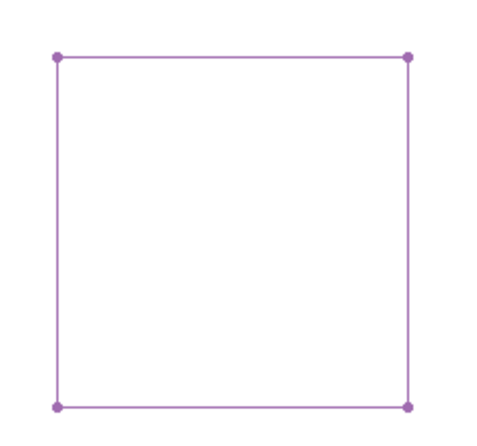
\includegraphics[width=1in]{cube2D.pdf}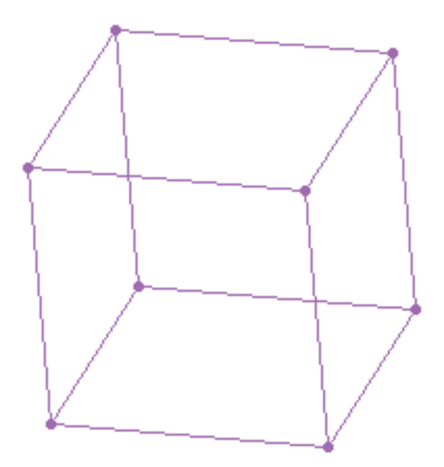
\includegraphics[width=1in]{cube3D.pdf}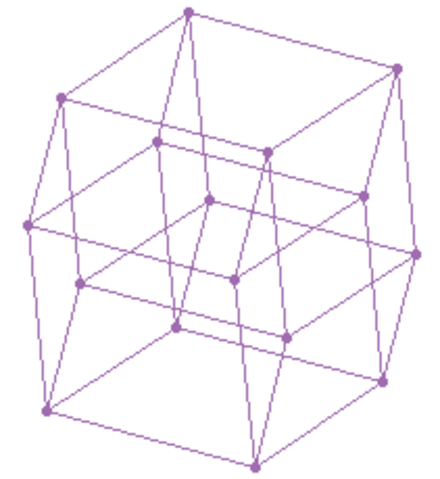
\includegraphics[width=1in]{cube4D.pdf}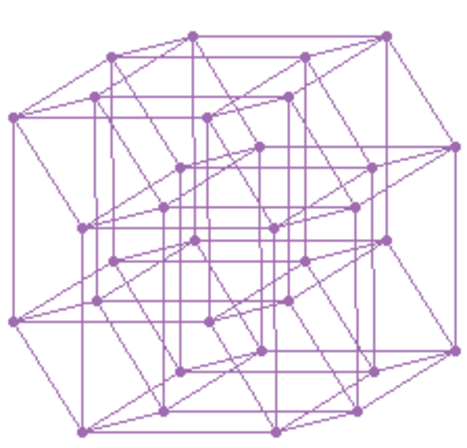
\includegraphics[width=1in]{cube5D.pdf}}
\caption{Wireframe cubes: 2-D, 3-D, 4-D, 5-D.}
\label{boxes}
\end{figure}

An alternative way to think of a high-dimensional cube is that it can
be considered to be all permutations of binary digits (0 and 1) in
$p$-D. A line is defined by two points: $(0)$, $(1)$. A square is
defined by four points: $(0,0)$, $(0,1)$, $(1,0)$, $(1,1)$, which are
all of the permutations of $0$ and $1$ in two columns, that is, the
Cartesian product of two lines. A 3-D cube is the Cartesian product of
two squares, and has all of the permutations of 0 and 1 in three
columns.

\subsection{Points on Vertices}~\label{cube-vertices}

The two different ways to define a high-dimensional cubes leads to two
different methods to create a $p$-D cube. Both methods yield the same
result, which is shown for $p=1,2,3$ in Table \ref{verticetable}.

\begin{itemize}

  \item {\bf Method 1:} Recursively double a lower-dimensional cube.
 
    Using the standard coordinate system, the base is 0 and 1. After
    establishing the base, we recursively double the base in the first
    column(s), and add an additional column containing a 0 in the
    first half of the rows and a 1 in the second half of the rows. The
    process is repeated $(p-1)$ times, to obtain a $p-$D cube.

\begin{verbatim}
cube.iterate <- function(p) {
     set <- rbind(0, 1)
     for (i in 1:(p-1)){
          set <- rbind(cbind(set, 0), cbind(set, 1))
     }
     set
} 
\end{verbatim}

  \item {\bf Method 2:} Generate all permutations of ${0, 1}$ in $p$ columns.
  
    This method takes advantage of an existing function in R,
    \code{expand.grid}. It produces all permutations by generating the
    Cartesian product of a set of vectors. For our purposes, the
    number of columns is not fixed, so we use \code{do.call}, to
    convert a function call of the form \code{x(a, b, c)} to
    \code{do.call(x, list(a, b, c))}, allowing specification of an
    arbitrary number of arguments.

  \begin{verbatim}
cube.permute <- function(p) {
  as.matrix(do.call(expand.grid, rep(list(c(0,1)), p)))
}
\end{verbatim}
\end{itemize}

\subsection{Completing the Wire Frame}

The wire frame for a cube draws the edges of the cube, that it is
connects all points that differ in one of the values, e.g. $(0,0,0)$
and $(1,0,0)$, or $(0,0,0)$ and $(0,1,0)$ for a 3-D cube. Each edge is
a vector of length $1$, and it is defined by specifying the row
numbers of the two corresponding elements of the vertex data, e.g. in
a 3-D cube $(2,4)$ would connect rows $2 (1,0,0)$ and $4
(1,1,0)$. Also edges are not ordered $(1,2)=(2,1)$, and we use just
one of the two, with the smaller number first. Here are three ways to
generate an edge set, the last being the most computationally
efficient but less intuitive. Table \ref{verticetable} gives vertex
and edge lists for $p=1, 2$ and $3$.

\begin{itemize}

  \item {\bf Method 1:} Distance of 1.
  
    The distance between all $p * (p - 1) / 2$ pairs of vertices is
    computed, and those pairs of vertices which have distance $1$ are
    returned. This is the simplest approach but obviously slow to
    compute as $p$ increases.

\begin{verbatim}
cube.edges.length1 <- function(cube) {
  a <- 2 ^ ncol(cube)
  cube.lines <- NULL
  for (i in 1:(a-1)) {
    for (j in (i+1):a) {
      d1 <- sum((cube[i, ]-cube[j, ])^2)
      if (d1==1) cube.lines <- rbind(cube.lines, c(i,j))
    }     
  }
  cube.lines
}
\end{verbatim}

  \item {\bf Method 2:} The binomial approach.
  
    This is faster to compute than the first method because it
    involves only a single loop over the cube vertices. For this
    approach to work, the vertices of the cube need to have been
    created using the methods described in
    Section~\ref{cube-vertices}. Each vertex, that has $c$ elements
    equal to 0, will be connected to $c$ other vertices, and we need
    to determine the row numbers for these other vertices. The row
    number for a corresponding connected vertex is obtained by adding
    2$^{(j-1)}, j=1,...,\#p$, if column $j$ contains 0, to the row
    number, $i, i=1,...,\#vertices-1$ of the originating vertex. For
    example, for a 3-D cube, the first vertex $(0,0,0)$ will be
    connected to vertices $2^0+1=2, 2^1+1=3, 2^2+1=5$.

\begin{verbatim}
cube.edges.binomial <- function(cube) {
  cube.lines <- NULL
  for (i in 1:(nrow(cube)-1)) {
    for (j in 1:ncol(cube)) {
      if (cube[i,j] == 0) {
        a <- 2 ^ (j - 1) + i
        cube.lines <- rbind(cube.lines, c(i,a))
      }
    }
  }
  cube.lines
}
\end{verbatim}

  \item {\bf Method 3:} Binary relationships.
  
    The final method is the most computationally efficient, but the
    least intuitive. Here we will use the fact that the vertices of
    the cube can be represented as binary numbers, e.g.  $(0, 1, 1) =
    011_2 = 3_{10}$. This allows us to both vectorize the code, and
    use the very fast C bitwise operations provided by the
    \pkg{bitops} package.

    The key insight is to note that edges connect vertices which have
    a single bit flipped. For example, $011$ connects to $111$, $001$
    and $010$ (vertex 3 connects to 7, 1, and 2). We can flip a single
    bit with the exclusive or function, $011 \oplus 100 = 111$, $011
    \oplus 010 = 001$, $011 \oplus 001 = 010$.  This leads to a fast
    and efficient method for generating the edges.

\begin{verbatim}
library(bitops)
cube.edges.binary <- function(p) {
  vertices <- 0:(2 ^ p - 1)
  from <- vertices[rep(1:length(vertices), each=p)]
  edges <- 2 ^ (0:(p-1))
  to <- bitXor(from, edges)
  cube.wires <- subset(data.frame(from, to), from < to) + 1
  cube.wires
} 
\end{verbatim}

\end{itemize}

\begin{table*}[htp]
  \centering
1-D:
\bigskip

\begin{tabular}{|l ||r|| r|}
\hline
row \# & 1 & edges \\
\hline
1 & 0 & 2\\
\hline
2 & 1 & \\
\hline
\end{tabular}
\bigskip

2-D:
\bigskip

\begin{tabular}{|l ||r|r|| r r|}
\hline
row \# & 1 & 2 & \multicolumn{2}{c|}{edges} \\
\hline
1 & 0 & 0 & 2 & 3\\
\hline
2 & 1 & 0 &  & 4 \\
\hline
3 & 0 & 1 &  4 & \\
\hline
4 & 1 & 1 &  & \\
\hline
\end{tabular}

\bigskip

3-D:
\bigskip

\begin{tabular}{|l ||r|r|r|| r r r|}
\hline
row \# & 1 & 2 & 3 & \multicolumn{3}{c|}{edges} \\
\hline
1 & 0 & 0& 0 & 2 & 3 & 5\\
\hline
2 & 1 & 0 & 0 & & 4 & 6\\
\hline
3 & 0 & 1 & 0 & 4 & & 7\\
\hline
4 & 1 & 1 & 0 & & & 8\\
\hline
5 & 0 & 0 & 1 & 6 & 7 & \\
\hline
6 & 1 & 0 & 1 & & 8 & \\
\hline
7 & 0 & 1 & 1 & 8 & & \\
\hline
8 & 1 & 1 & 1 & & & \\
\hline
\end{tabular}
\caption{Cube Vertices and Edges.}
\label{verticetable}
\end{table*}

\subsection{Solid Cube}

A solid cube has points in the interior (Figure~\ref{solcube}). It is
easy to generate, using either random sampling or a fixed grid.

\begin{figure}[ht]
\centerline{
\begin{tabular}{c c c}
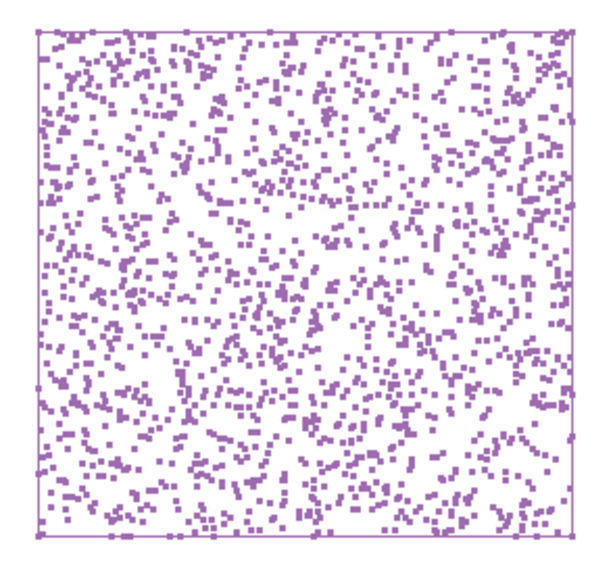
\includegraphics[width=1in]{cube-2-solid.pdf} & 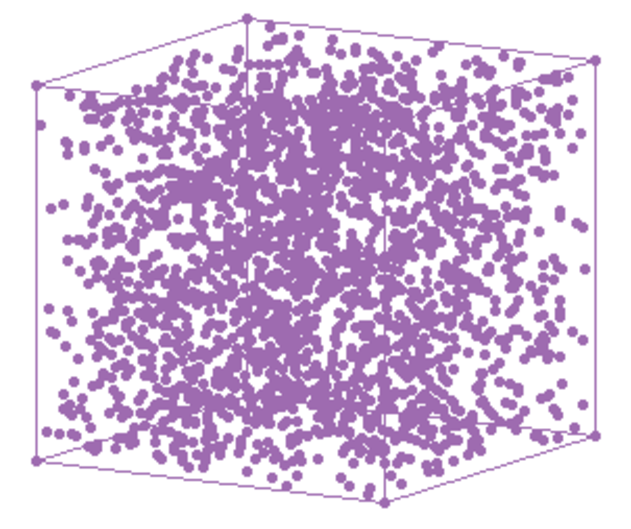
\includegraphics[width=1in]{cube-3-solid.pdf} & 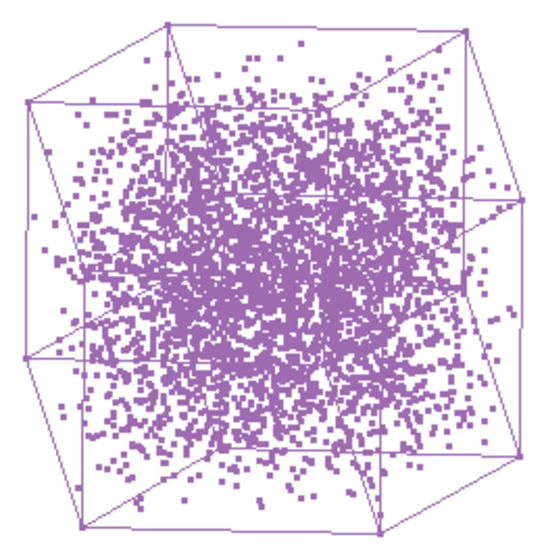
\includegraphics[width=1in]{cube-4-solid.pdf}\\
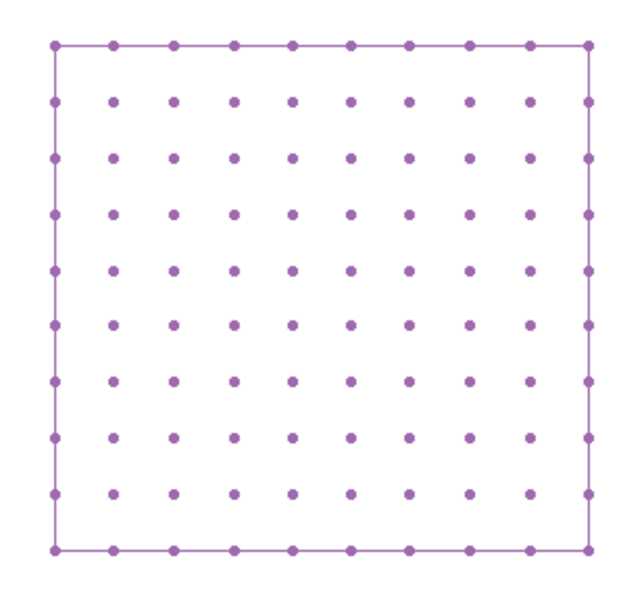
\includegraphics[width=1in]{cube-2-solideq-9.pdf} & 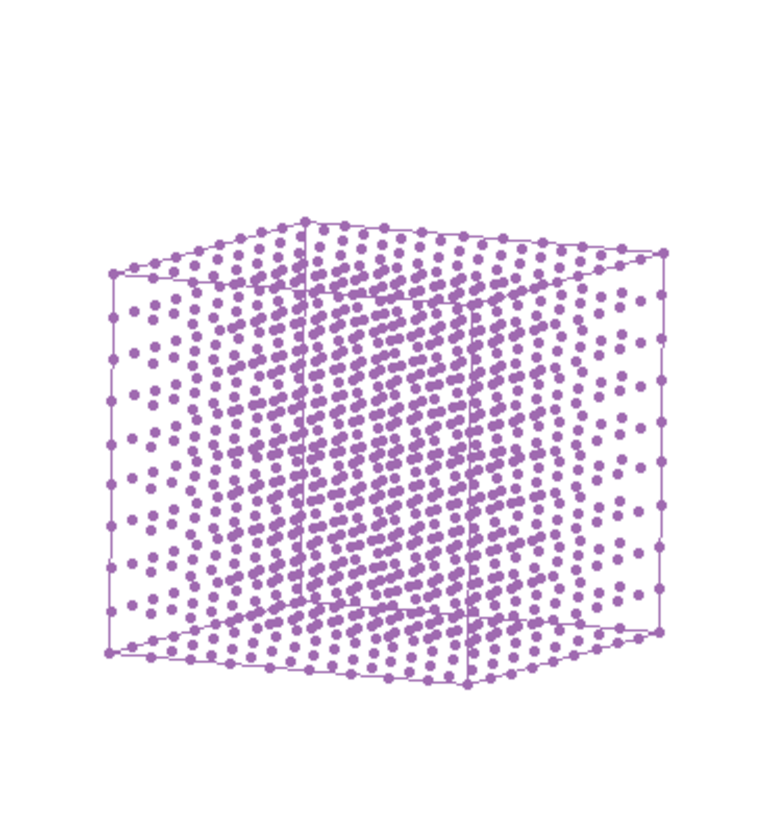
\includegraphics[width=1in]{cube-3-solideq-9.pdf} & 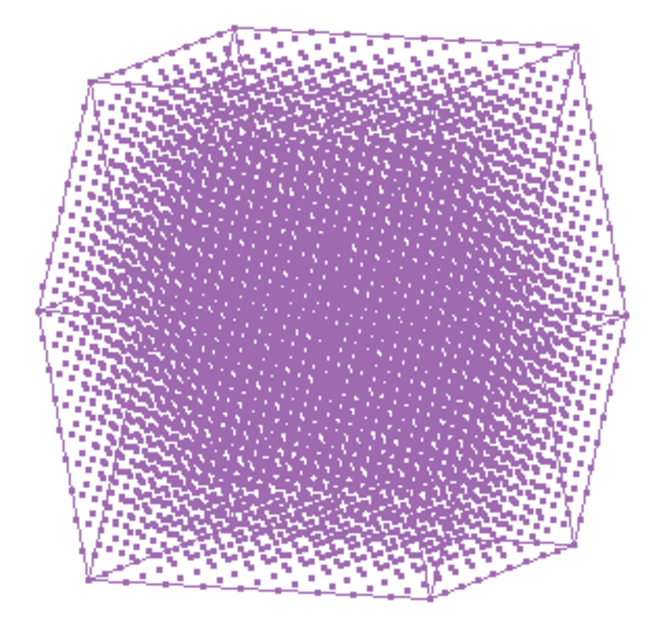
\includegraphics[width=1in]{cube-4-solideq-9.pdf}
\end{tabular}
}
\caption{Solid cubes in 2-D, 3-D, and 4-D (top) random samples from
  $p$ uniform distributions (bottom) fixed grid.}
\label{solcube}
\end{figure}

\begin{itemize}

  \item {\bf Method 1:} Random uniform.
  
    The R function \code{runif} function generates samples from a
    uniform distribution between 0 and 1. Generating $p$ random
    uniform values creates a $p$-dimensional vector corresponding to a
    point inside a $p$-dimensional cube. The number of points needed
    to make the cube appear solid increases as $p$ increases. The
    volume of the cube doubles with each dimension. For example, a 3-D
    cube with side length 2 has the volume $2^3=8$, and a 4-D cube
    with the same side length has the volume $2^4=16$. Thus the number
    of points must be at least doubled for each increase in
    dimension. In our function, we use a base of 850 points. The total
    number of points is capped at 50000 points for speed of viewing.

\begin{verbatim}
cube.solid.random <- function(p, n = 850 * 2^p) {
  x <- matrix(runif(n*p), ncol = p)
  colnames(x) <- paste("X", 1:p, sep="")
  x
}
\end{verbatim}

  \item {\bf Method 2:} Equidistant.
  
    A solid cube can also be generated with equidistant points. As
    with the second vertex generation method the \code{expand.grid}
    function is used. The input $n$ allows the number of grid points
    to be varied.

\begin{verbatim}
cube.solid.grid <- function(p,n) {
  grid <- list(seq(0, 1, length = n))
  do.call(expand.grid, rep(grid, p ))
}
\end{verbatim}
\end{itemize}

There are advantages and disadvantages.  The first method, random
points, produces a solid cube that looks more solid, but as $p$
increases points near the vertices become more scarce.  With
equidistant points the filled cubes look more structured, and there
are always points near the vertices.

\subsection{Hollow Cube}

The ``face'' of a cube is a surface that is one dimension lower than
that of the cube.  For example, a face of a 3-D cube is a 2-D square
and a face of a 4-D cube is a 3-D cube. To generate points on the
faces of a cube, random points are created in all dimensions except
one. The last dimension is given the value of $0$ or $1$, to create
the opposing faces.

For a 3-D cube, the $X_1$ and $X_2$ components of the cube are given
random values and the $X_3$ components would be set to 0 in the first
half and 1 in the second half. The process would then be repeated for
the remaining columns, as shown in Figure \ref{faces}. This will
create six 2-D squares which form the faces of a 3-D cube.

Figure \ref{4faces} shows the faces of a 4-D cube being built. The
left side plot shows the first pair of faces, a solid 3-D cube in
$X_1, X_2, X_3$, with fixed values on the fourth dimension $X_4$. The
subsequent plots show the remaining faces.

\begin{figure}[ht]
  \centering
  \begin{tabular}{c c c}
    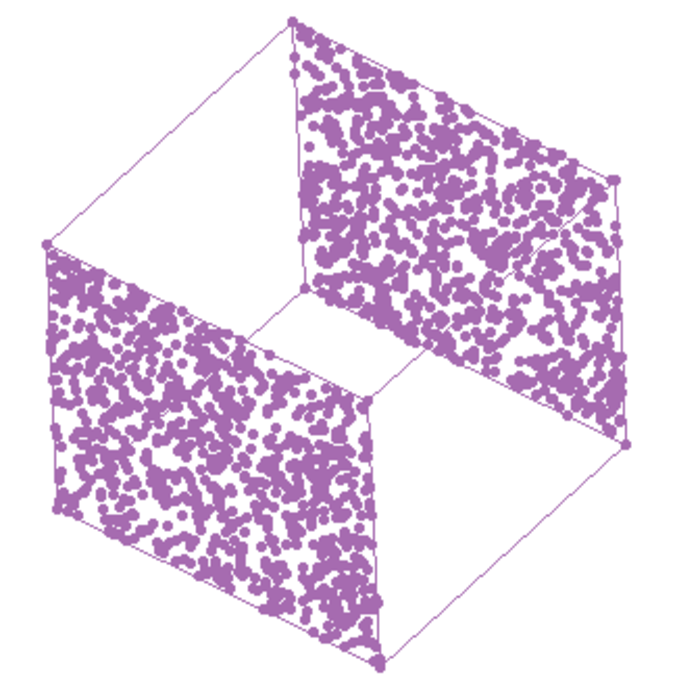
\includegraphics[width=1in]{cube-x.pdf} &
    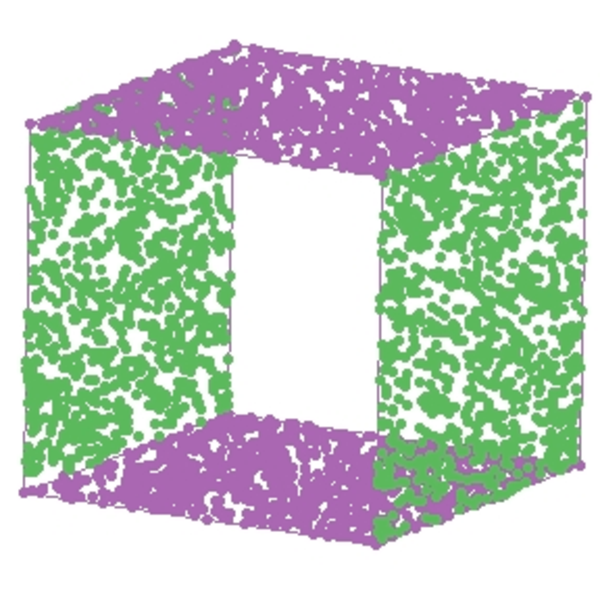
\includegraphics[width=1in]{cube-x-y.pdf} &
    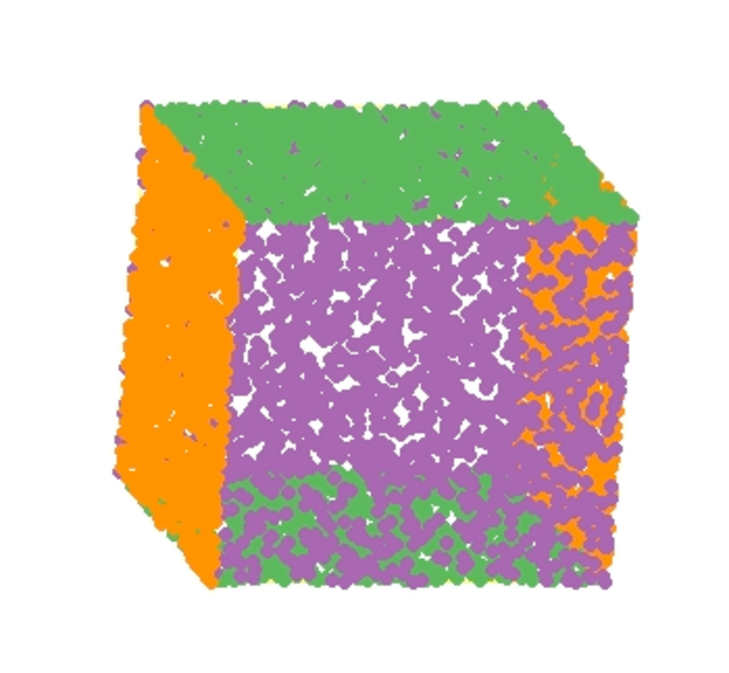
\includegraphics[width=1in]{cube-x-y-z.pdf} 
  \end{tabular}

  \caption{Faces of a 3-D cube, $X_3$, $X_2$\&$X_3$,
      $X_1$\&$X_2$\&$X_3$.}
  \label{faces}
\end{figure}

\begin{figure}[ht]
\centerline{
\begin{tabular}{c c c c}
  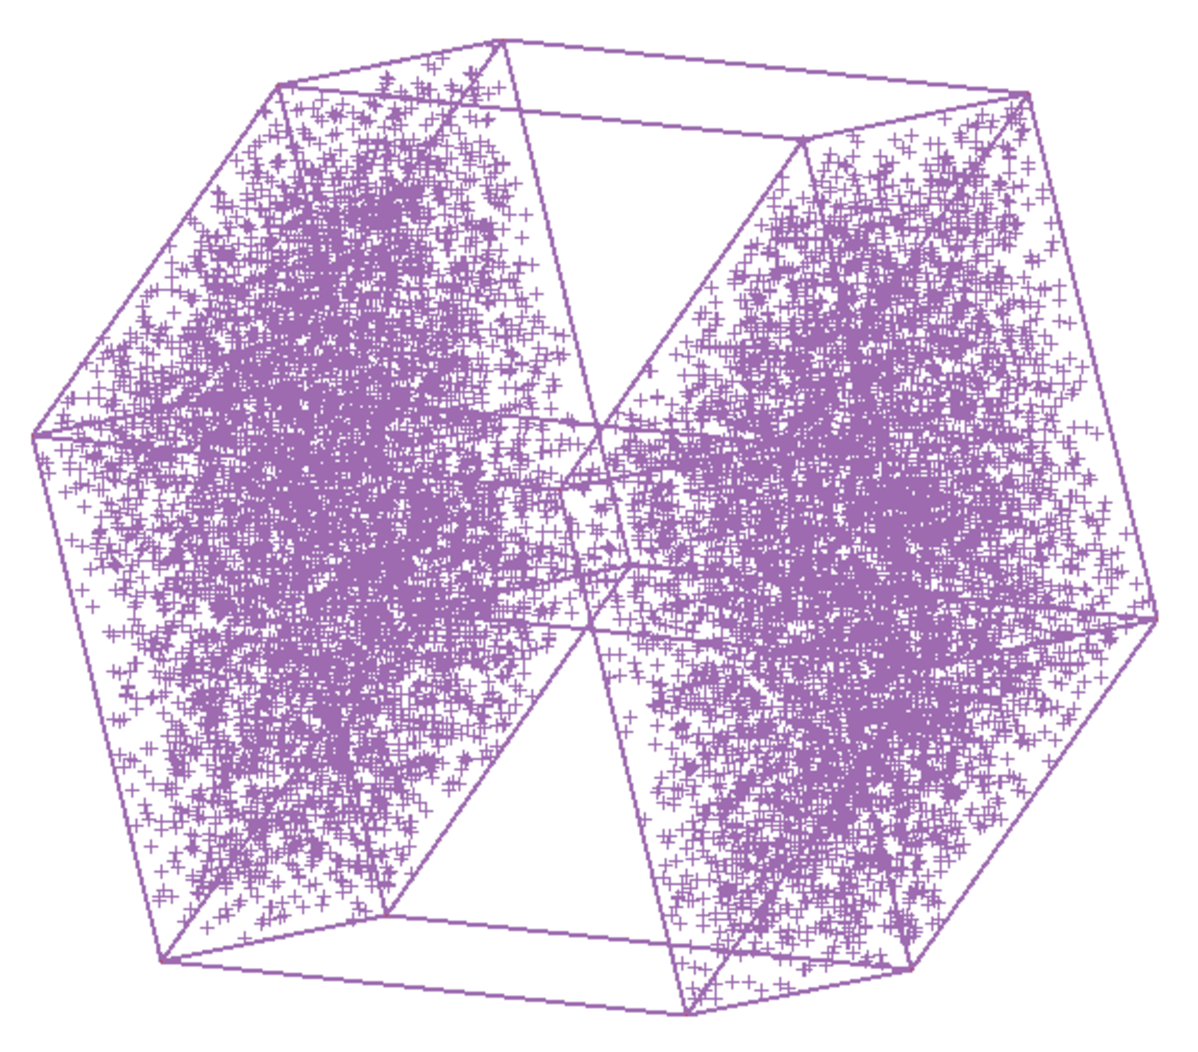
\includegraphics[width=1in]{cube-4-face-1-1.pdf} & 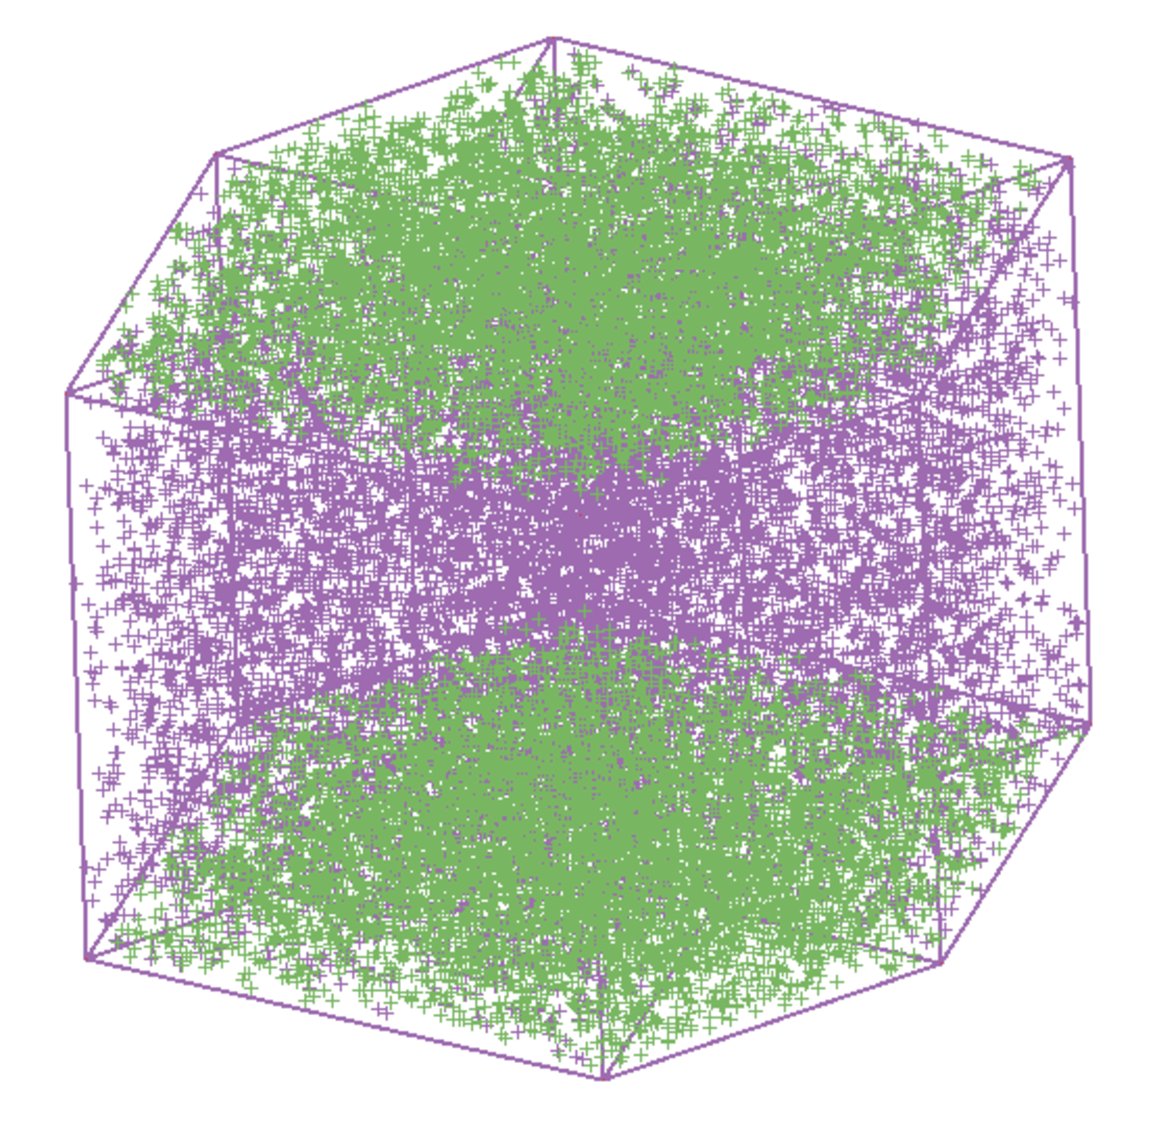
\includegraphics[width=1in]{cube-4-face-2-1.pdf} & 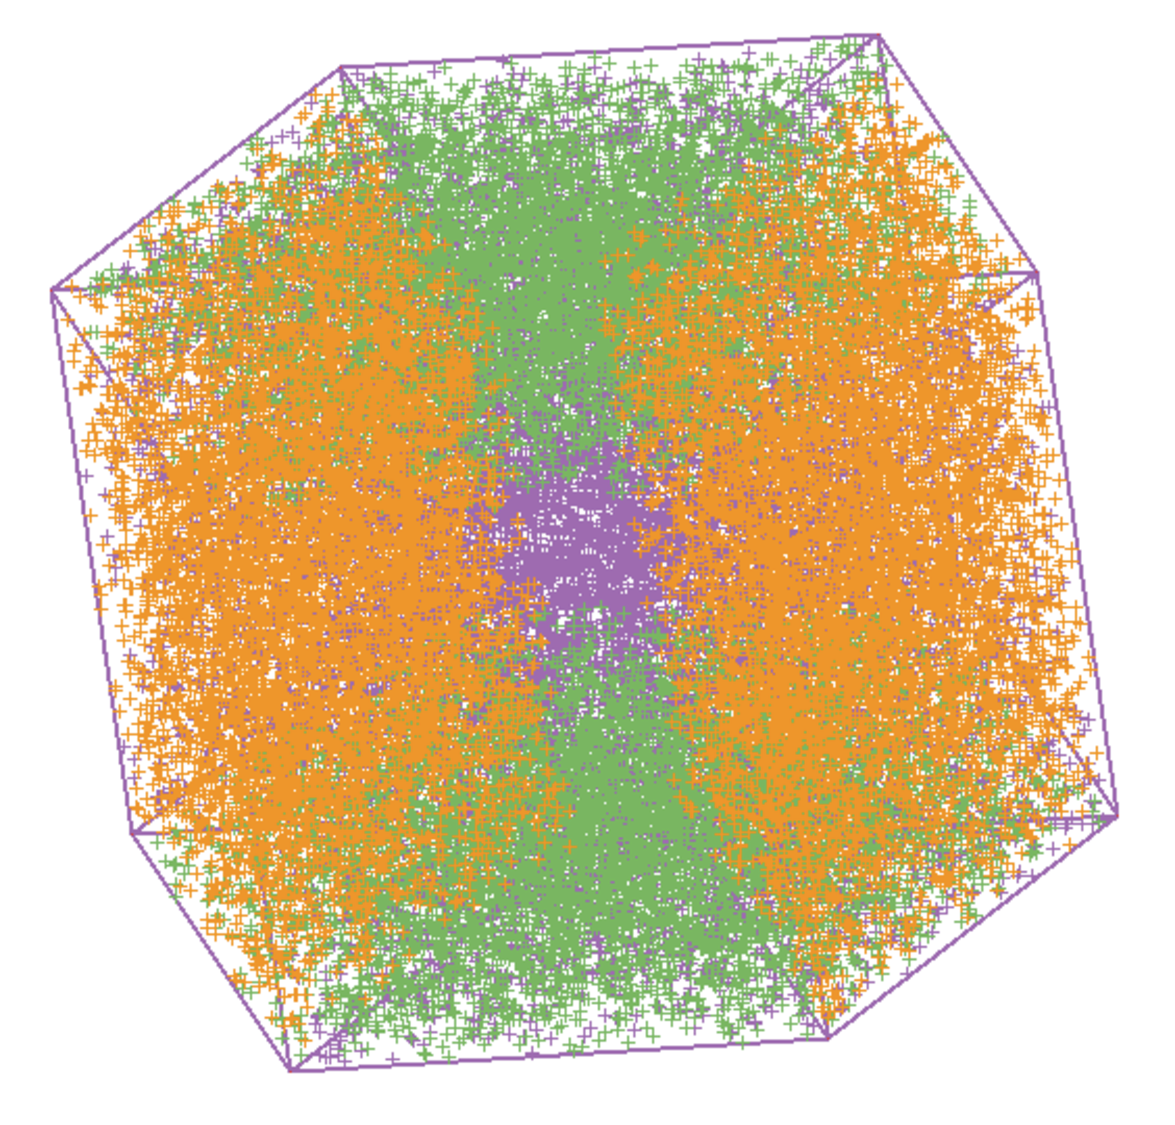
\includegraphics[width=1in]{cube-4-face-3-1.pdf} &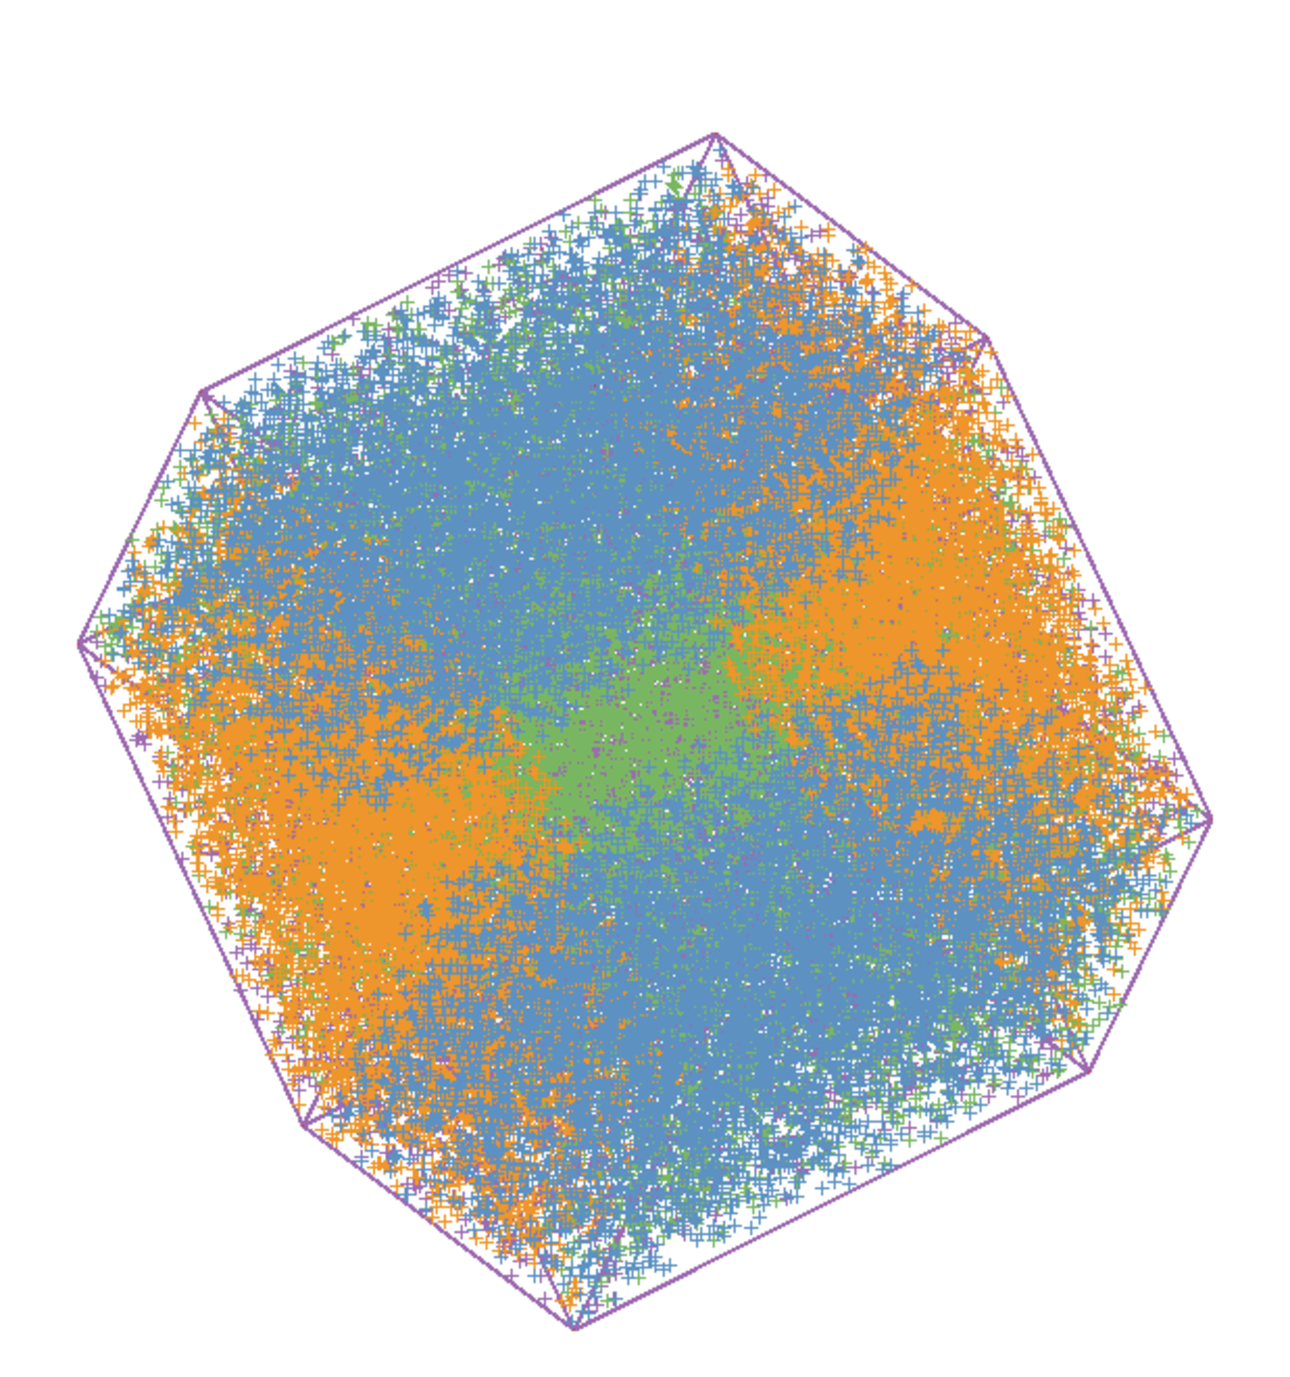
\includegraphics[width=1in]{cube-4-face-4-1.pdf}
\end{tabular}
}
\caption{Faces of a 4-D cube, $X_4$, $X_3$\&$X_4$, $X_2$\&$X_3$\&$X_4$,
  $X_1$\&$X_2$\&$X_3$\&$X_4$.}
\label{4faces}
\end{figure}

\begin{figure}[ht]
\centerline{
\begin{tabular}{|c|c|c|c|}
\hline
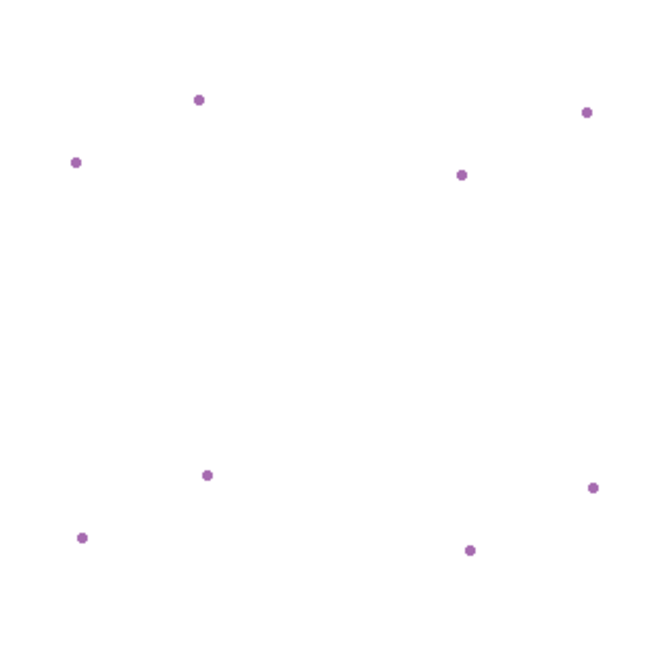
\includegraphics[width=1in]{cube-3-vert.pdf} & 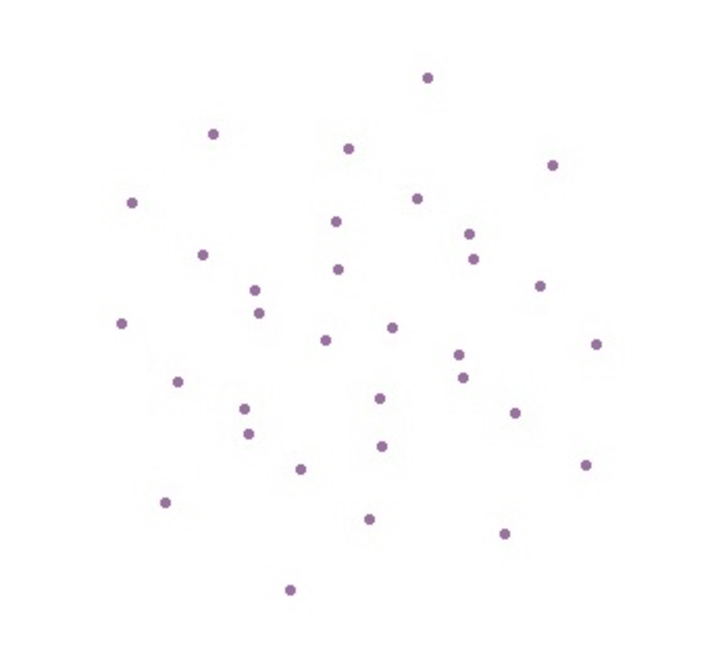
\includegraphics[width=1in]{cube-5-vert.pdf} & 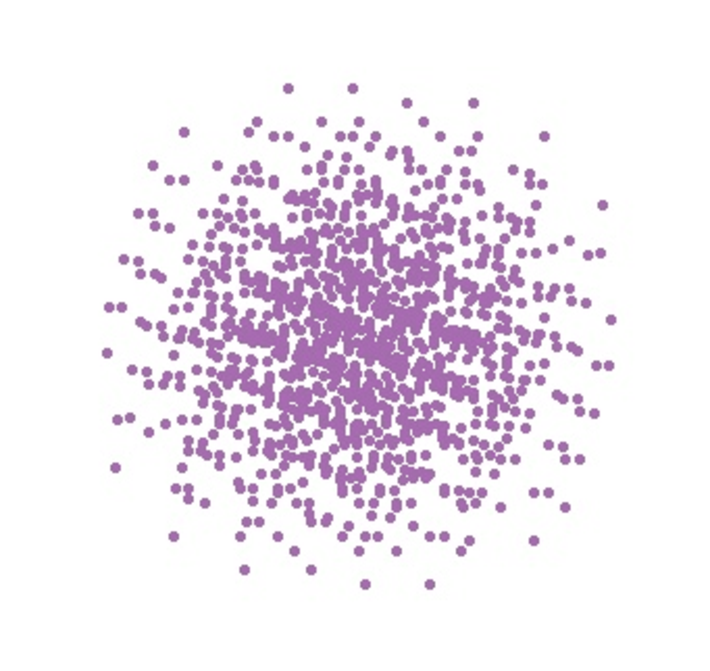
\includegraphics[width=1in]{cube-10-vert.pdf} & 
\includegraphics[width=1in]{cube-15-vert.pdf}\\
\hline
\end{tabular} 
}
\caption{Vertices of cubes: 3-D, 5-D, 10-D, and 15-D. They look more
  rounded as the dimension increases.}
\end{figure}

\subsection{High-D Cubes Look Spherical!}

As the dimension increases the shape the cube takes in a 2-D
projection looks more rounded than square. The reason is explained in
\citet{DF84} and is related to the Central Limit Theorem. When we use
a tour to visualize high-dimensional data we examine low-dimensional
projections.  Consider the axes for a $p$-dimensional space labeled as
$X_1, ..., X_p$. A 1-D projection is generated by taking a linear
combination of these axes, such as $a_1X_a+...+a_pX_p$. The squared
values of $a_j, j=1, ..., p$ are constrained to sum to 1. As $p$
increases, the combining the values operates like averaging the values
in many dimensions, resulting in views that look Gaussian. Another way
to think about it is that we are looking at rotated cubes rather than
a cube through its square face and this gets increasingly rounded as
the dimension of increases. (More details about tours can be found in
many papers, including \cite{BCAH05}, \cite{ClBW07}).


\section{Spheres}

A sphere can be described as $\{X: X_1^2+\dots + X_p^2 \leq 1\}$, all
points within a fixed radius of zero.  A hollow sphere is the set of
points with radius equal to 1.

\subsection{Hollow Sphere}

To generate points uniformly distributed on the surface of a sphere we
use a trick: First, generate a random vector from a multivariate
standard normal distribution and then normalize its length. The top
row of Figure \ref{cfb} shows the results.

\begin{verbatim}
norm.vec <- function(x) {
  x <- x / sqrt(sum(x ^ 2))
  x
}

sphere.hollow <- function(p, n = p * 500) {
  x <- matrix(rnorm(n * p), ncol = p)
  t(apply(x, 1, norm.vec))
}
\end{verbatim}

\begin{figure}[ht]
\centering
\begin{tabular}{c c c}
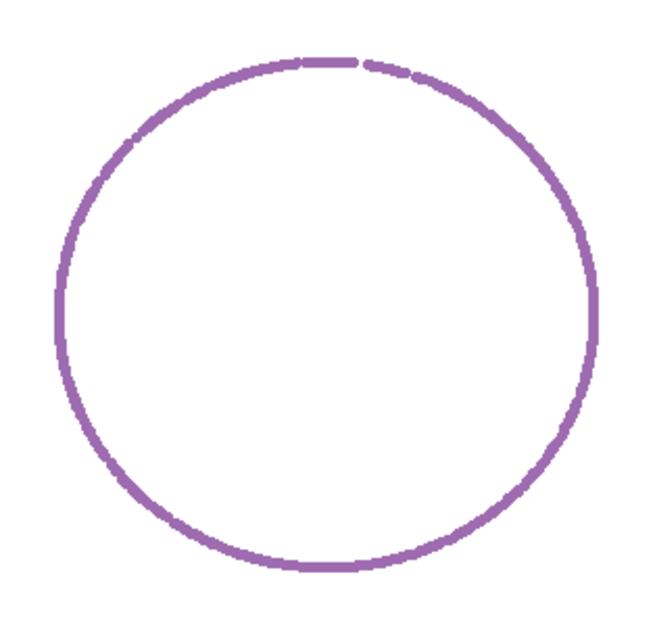
\includegraphics[width=1in]{sphere-2.pdf} 
&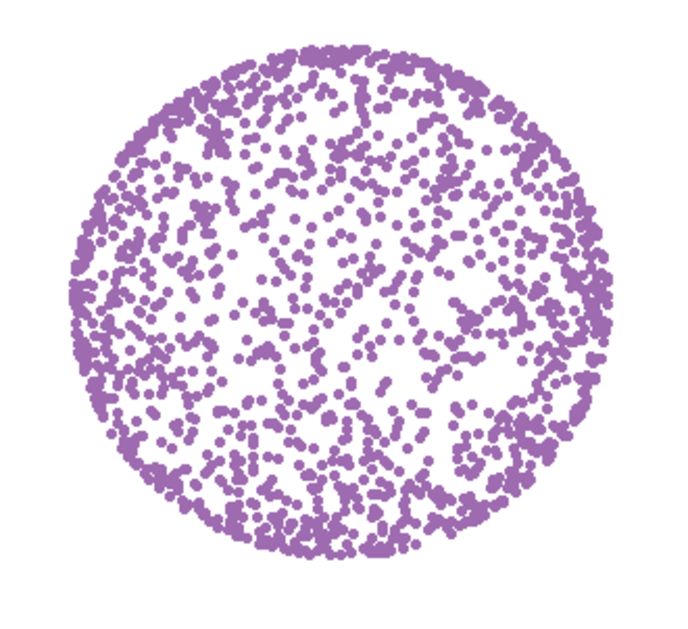
\includegraphics[width=1in]{sphere-3.pdf} 
&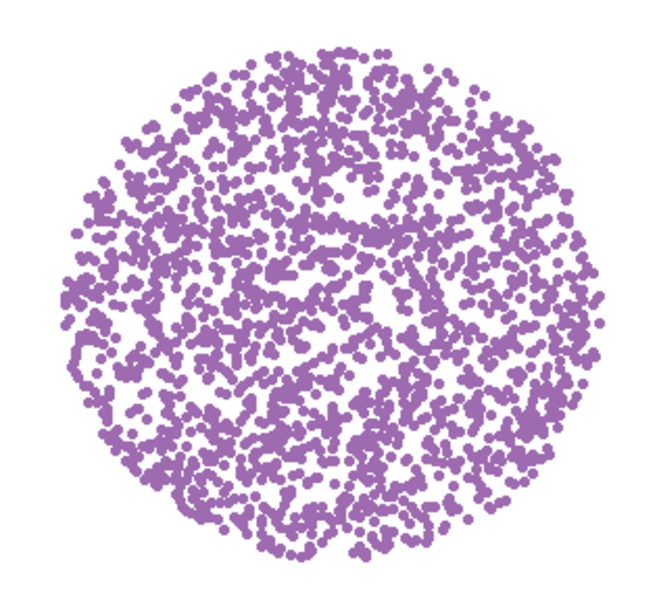
\includegraphics[width=1in]{sphere-4.pdf}
\\
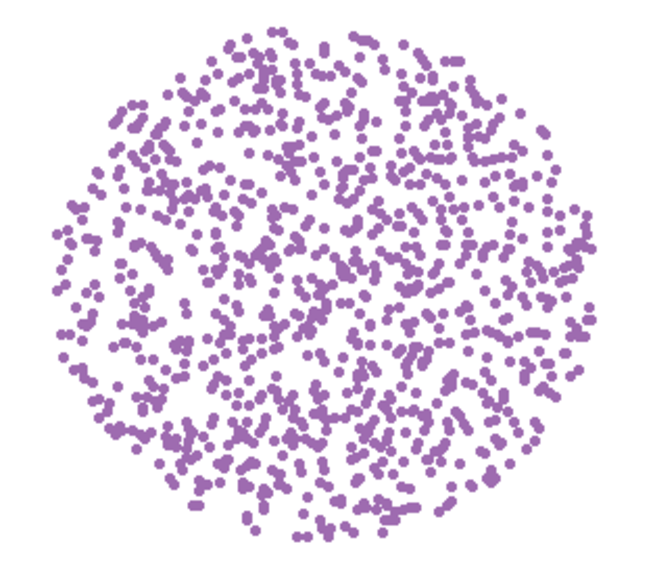
\includegraphics[width=1in]{sphere-2-solid.pdf} 
&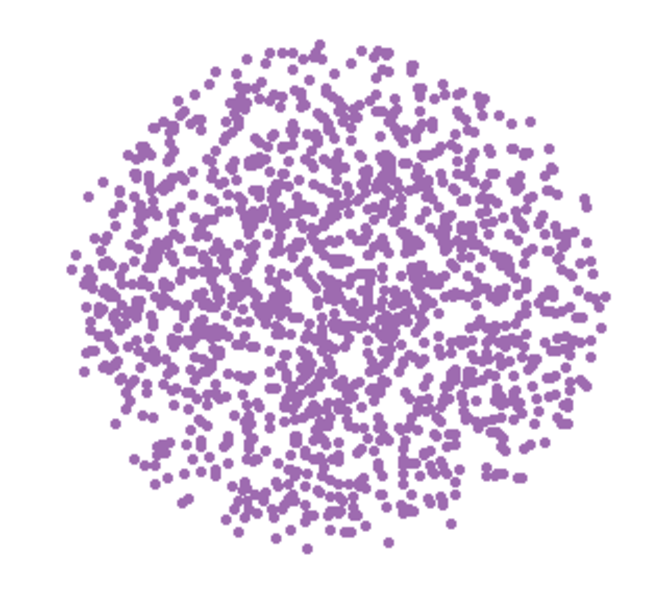
\includegraphics[width=1in]{sphere-3-solid.pdf} 
&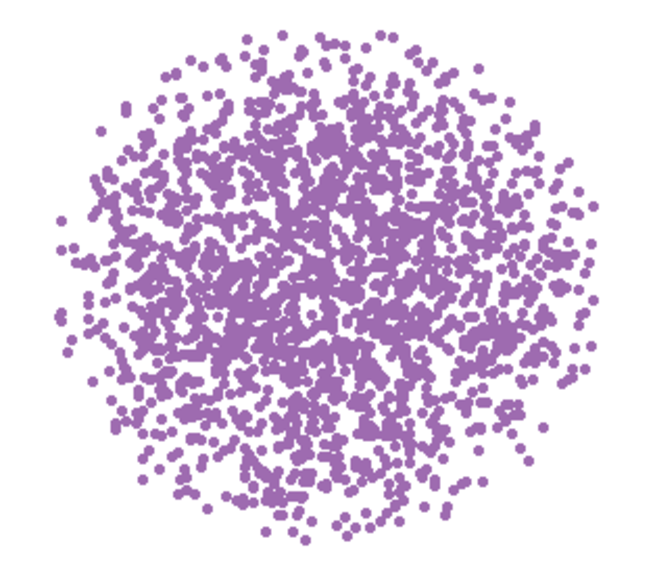
\includegraphics[width=1in]{sphere-4-solid.pdf} 
\end{tabular}
\caption{Hollow (top row) and solid spheres (bottom row) for 2-D, 3-D,
  4-D.}
\label{cfb}
\end{figure}

\subsection{Don't Reject the Solid Sphere!}

Solid spheres could be generated in much the same way as solid cubes; use
random points to fill the object. While the solid cube fills the box,
the sphere's points are inside a radius of 1 from the center. A simple
approach would be to use a rejection method: generate points in the
solid cube and discard those with radius more than 1. This is
problematic as $p$ increases. Most points will eventually be rejected.
For example, to generate the points of a 3-D sphere, around 50\% of
the points are kept, but for a 10-D sphere only 0.25\% of the points
are kept. The space in the corners of the box, outside the sphere
increases dramatically with $p$.

The approach we used is a minor modification to the method used to
generate a hollow sphere. Figure \ref{cfb} illustrates the
process. The vector length is randomly sampled from a uniform
distribution on $(0,1)$ (left plot). The result is raised to the power
$1/p$ to adjust for the volume increase with $p$, resulting in points
spread evenly throughout the inside of the sphere (middle plot).
Taking the sphere to the $1/p$ power may seem ad hoc, but the
operation ensures that the density uniform within the sphere. To see
this, compare circles of radius 1 and 2 (right plot).  The area of the
smaller circle equals $\pi =  1^2\pi $.  The area of the whole
circle equals $ 4 \pi = 2^2 \pi $. This is four times as large, but
only twice the radius.  Thus without accounting for radial distance
more points will be generated closer to the center than is warranted
by the area.  Raising the vector length to the power $1/p$, 1/2 in our
example, corrects for the volume.

\begin{verbatim}
sphere.solid.random <- function(p, n = p * 500) {
  sphere.hollow(p, n) * runif(n) ^ (1/p)
}
\end{verbatim}

\begin{figure}[ht]
\centering
\begin{tabular}{c c c}
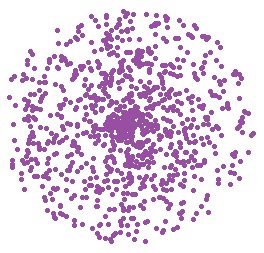
\includegraphics[width=1in]{sphere-2-bad.jpg} 
&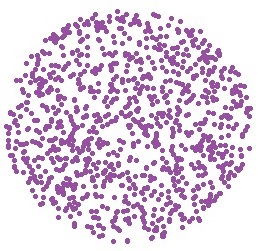
\includegraphics[width=1in]{sphere-2-good.jpg} 
&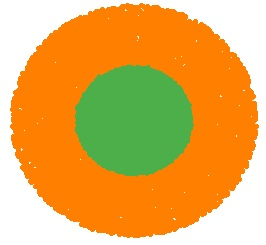
\includegraphics[width=1in]{sphere-2-1and2.jpg}
\end{tabular}
\caption{Solid sphere in 2-D: (left) generated randomly results in an
  over-concentration of points in the center, (middle) adjusted for
  volume generates a uniform distribution inside the sphere, and
  (right) comparison of areas of circles of radius 1 and 2.}
\label{cfb}
\end{figure}

\section{Simplexes}

Simplexes are one of the simplest objects to create and view. A $p$-D
simplex is a shape that lives in one dimension less than $p$. It has
vertices corresponding to the coordinate axes. The simplex vertices
are then projected, using a Helmert matrix, into the
$(p-1)$-dimensional space in which it exists.

\begin{figure}[ht]
\centerline{
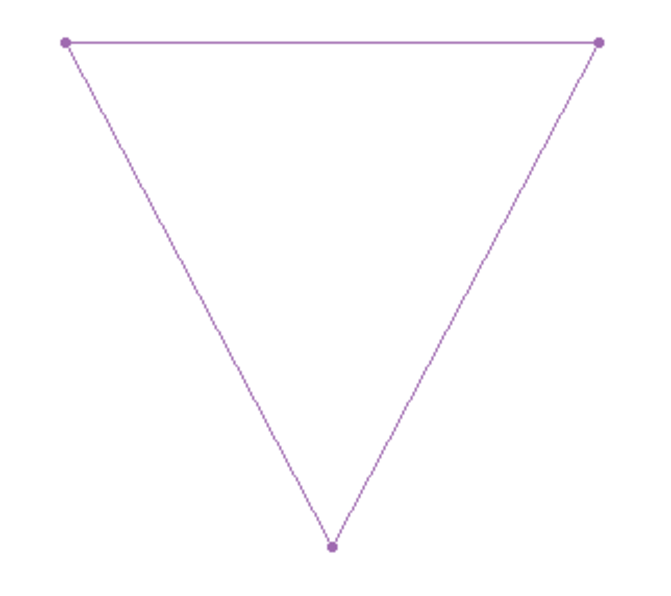
\includegraphics[width=1.2in]{simplex2.pdf}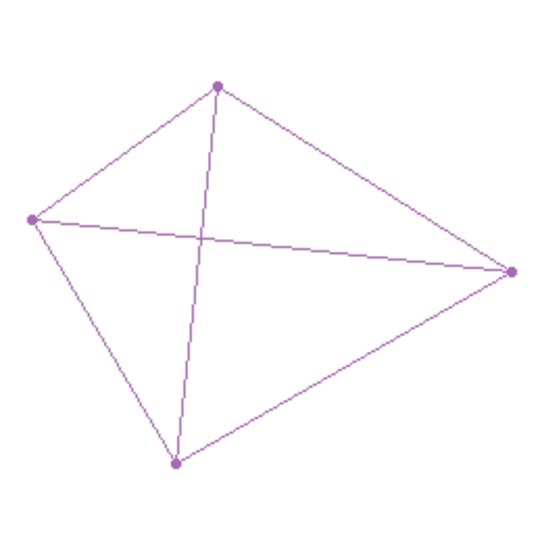
\includegraphics[width=1.2in]{simplex3.pdf}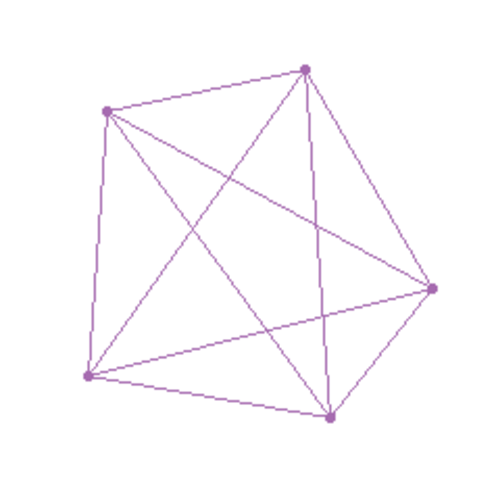
\includegraphics[width=1.2in]{simplex4.pdf}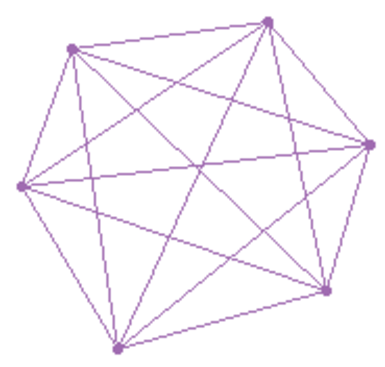
\includegraphics[width=1.2in]{simplex5.pdf}}
\caption{Wireframe simplexes: 2-D, 3-D, 4-D, 5-D.}
\end{figure}

For example, a 3-D simplex has vertices at (1,0,0), (0,1,0), (0,0,1),
which are reduced by the Helmert transformation to points a 2-D
equilateral triangle, (0.7071,0.4082), (-0.7071,0.4082), (0.0000,
-0.8165).

\begin{verbatim}
helmert <- function(d) {
  helmert <- rep(1/sqrt(d), d)
  for(i in 1:(d-1)){
    x <- rep(1/sqrt(i*(i+1)), i)
    x <- c(x, -i/sqrt(i*(i+1)))
    x <- c(x, rep(0, d - i - 1))
    helmert <- rbind(helmert, x)
  }
  helmert
}

simplex <- function(p) {
  x <- diag(p)
  # center simplex
  x <- x - matrix(1/p, p, p) 
  hm <- helmert(p) 
  final <- (x %*% t(hm))[,-1]
  final
}
\end{verbatim}

The wire frame for a simplex connects ever point to every other point, and can
be computed in just two lines of code, following method 2 of the cube
vertices. It makes a list of all combinations of each row number and then
removes the lines that connect a point to itself.

\begin{verbatim}
simplex.wires <- function(simplex) {
  wires <- do.call(expand.grid, 
    list(c(1:nrow(simplex)),c(1:nrow(simplex))))
  wires[!wires[,1]==wires[,2],]
}
\end{verbatim}

\section{Polyhedra}

A polyhedron is a three dimensional object that contains straight
edges and has flat faces. Our polyhedra data comes from George
W. Hart's website \citep{GeorgeVP}. Hart's website contains an
extensive collection of polyhedra, ranging from Platonic Solids to
Stellations of the Rhombic Triacontahedron. In our data sets, we used
the information from Platonic Solids, Kepler-Poinsot Polyhedra,
Archimedean Polyhedra and its duals, Prisms. The data was reformatted
from VRML, into the XML. The vertices and wire frames from separate
files were compiled into tables. Some reformatting of edges was also
necessary.

\begin{figure}[ht]
\centerline{
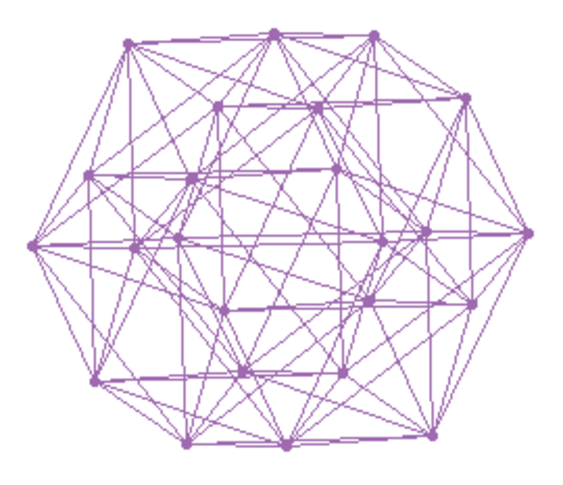
\includegraphics[width=1.2in]{24-cell.pdf}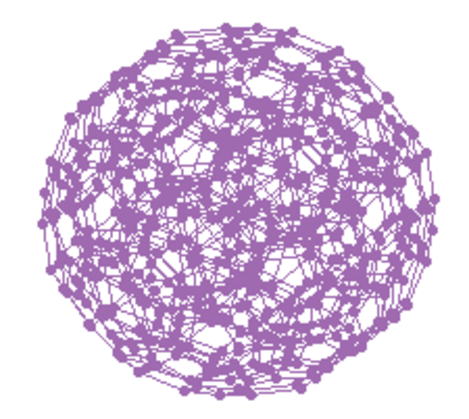
\includegraphics[width=1.2in]{120-cell.pdf}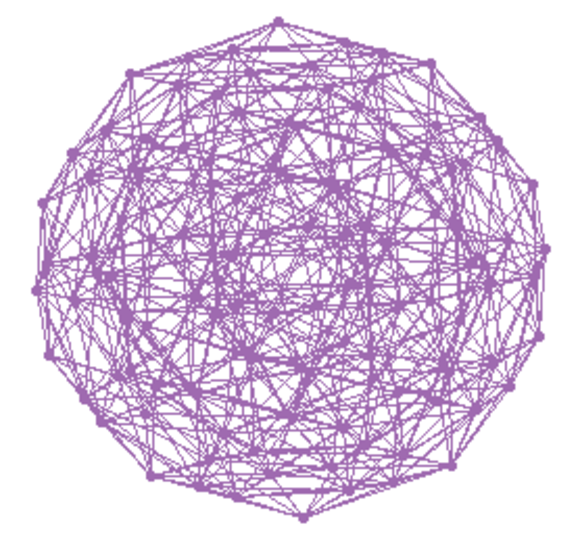
\includegraphics[width=1.2in]{600-cell.pdf}}
\caption{24-Cell, 120-Cell, and 600-Cell.}
\end{figure}

\section{Surfaces and Curves}

Paul Bourke's website \citep{PBCurves} has equations for generating
several famous objects, including the Mobius Strip, Steiner's Roman
Surface and the Klein Bottle. It is interesting to see how each object
twists onto itself.  R functions based on these equations were written
to produce each object.  Each object was rendered by points on the
surface. For each shape a set of random angles was generated to seed
the equations, generating points on the surface.  For some of the
objects, to view the object in its familiar form the limits for each
variable need to be equal, see Section \ref{notes}.

\begin{figure}[ht]
\centerline{

\includegraphics[width=1.2in]{mobius.pdf}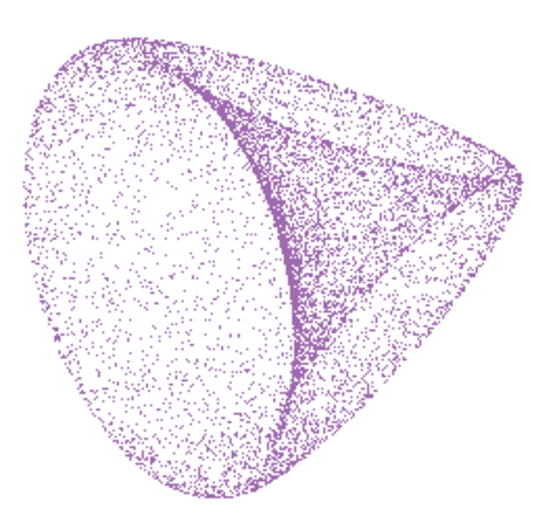
\includegraphics[width=1.2in]{roman.pdf}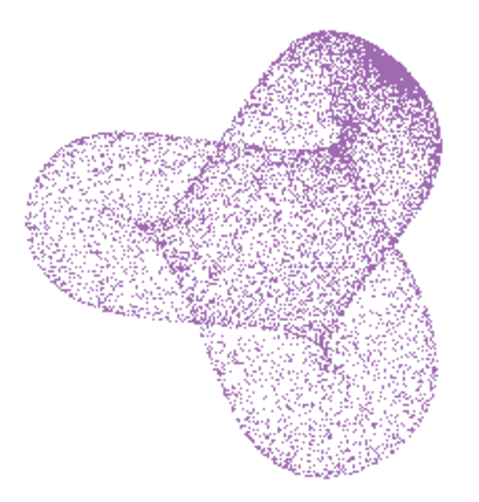
\includegraphics[width=1.2in]{boy-surface.pdf}}
\caption{Mobius strip, Steiner's roman surface, and Boy's surface.}
\end{figure}

\section{Polytopes}

A polytope is a generalized term of a geometric shape in any
dimension. A polygon is a 2-D polytope. A polyhedron is a 3-D
polytope. A polychoron is a 4-D polytope. Beyond that we typically use
polytope to refer to any $p$-gon.  Our polychoron data comes from Paul
Bourke's website \citep{PBPlatonic}, where there is information some
objects that we have already covered hypercube, simplex, and new
objects, 24-cell, 120-cell, 600-cell.  The explanations of these
polytopes is very clear. We've reformatted the data into XML files
defining vertices and edges for each of the shapes.

\section{Tori}

A ``doughnut'' torus is known as a ring torus. Paul Bourke's website
\citep{Pa90} on ``The Torus and Super Torus'' provides the
inspiration. The website explains how the 3-D torus is made.

It also contains information that we used to develop the process of
building high-dimensional tori.  Figure \ref{ringtorus} shows this
process: a small circle follows a larger circle, creating a
doughnut. The points for the torus are formed by polar coordinates.

\begin{figure}[ht]
\centerline{
\begin{tabular}{c c c}
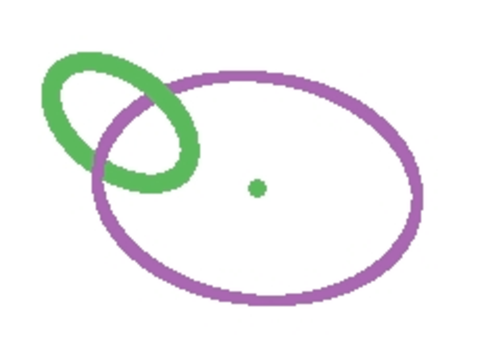
\includegraphics[width=1in]{torus-ring-3-2nd-1.pdf} & 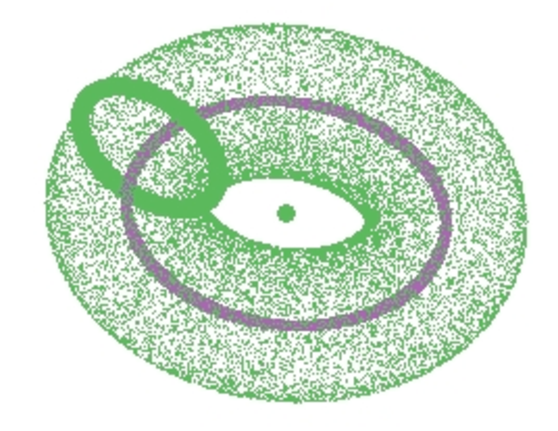
\includegraphics[width=1in]{torus-ring-3-2nd-2.pdf} & 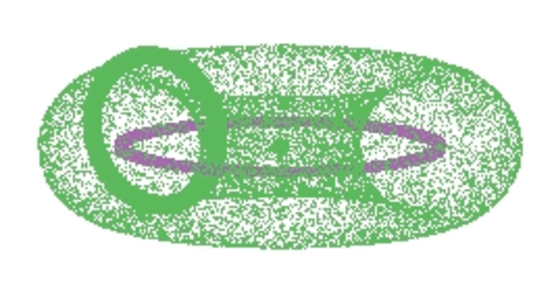
\includegraphics[width=1in]{torus-ring-3-2nd-3.pdf}   \\ 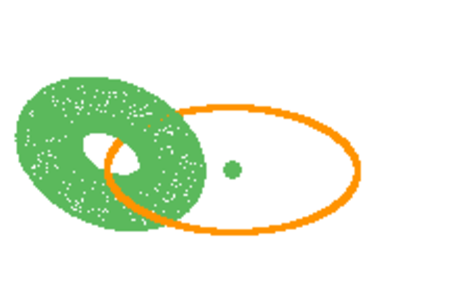
\includegraphics[width=1in]{torus-rings-4-2.pdf} &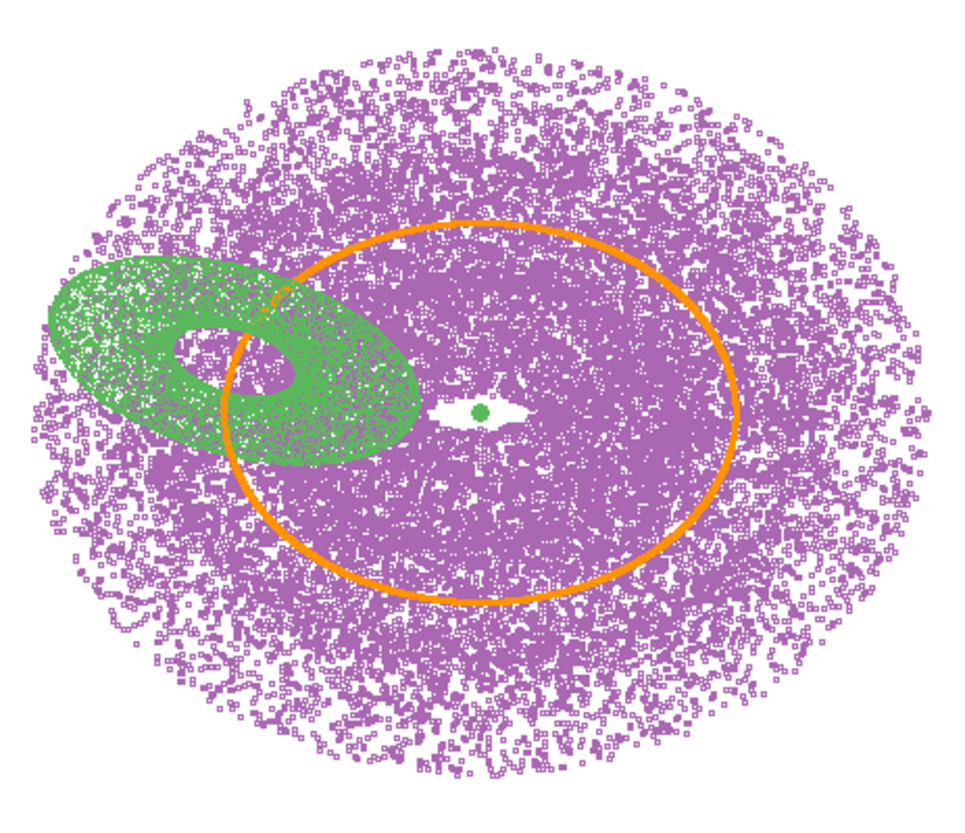
\includegraphics[width=1in]{torus-rings-4-with-torus-2.pdf}&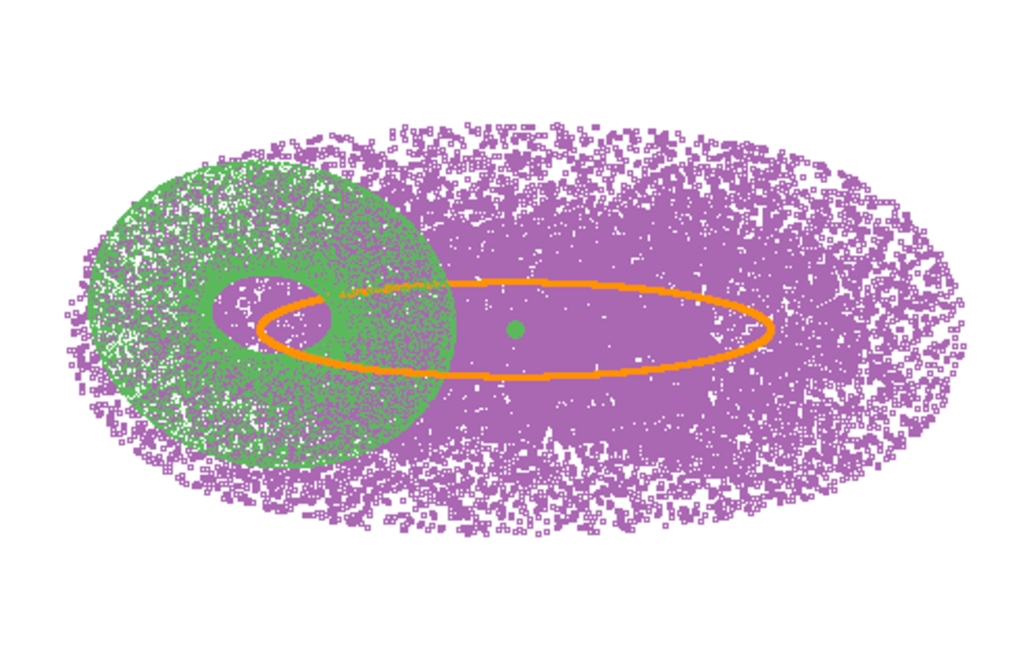
\includegraphics[width=1in]{torus-rings-4-with-torus-1.pdf}
\end{tabular}
}
\caption{Generating a torus: 2-D to 3-D, and 3-D to 4-D.}
\label{ringtorus}
\end{figure}

To produce a 4-D torus, a 3-D torus is rotated around a circle into
the fourth dimension (Figure \ref{ringtorus} bottom row).  This torus
still has a hole in the center.  A way to think about the process is a
recursive circle system. For a 3-D torus, the smaller radius circle
follows the larger radius circle. For a 4-D torus, a 3-D torus an even
larger radius circle.  That is, the lower-dimensional torus is
translated a fixed distance and rotated about a \textit{new} axis
perpendicular to the axis of the hole. The next two sections describe
the process in detail.

\begin{figure}[ht]
\centerline{
\begin{tabular}{c c c c}
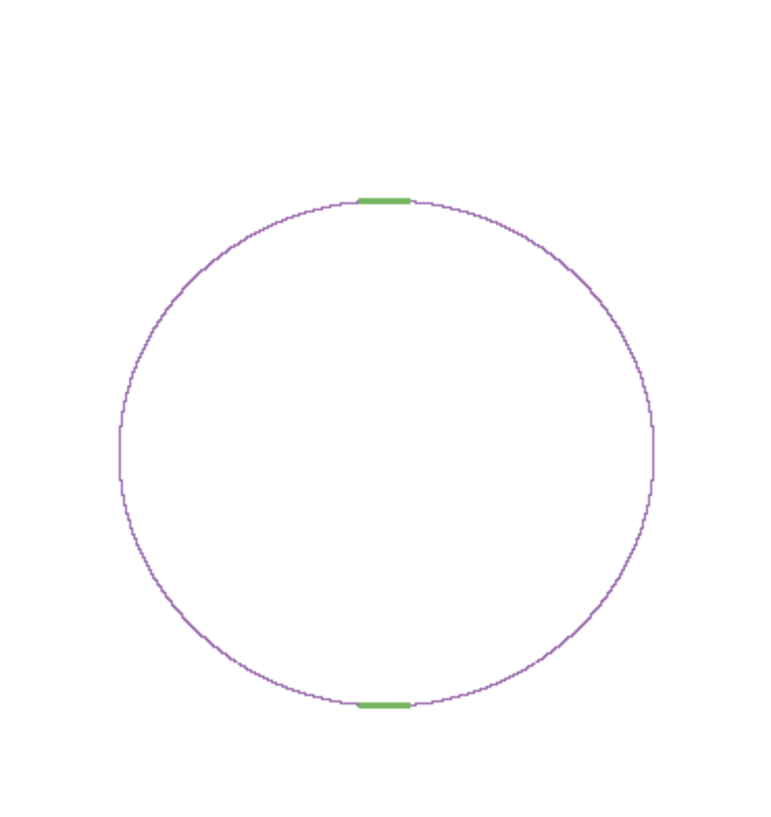
\includegraphics[width=1in]{torus-2-50k.pdf} & 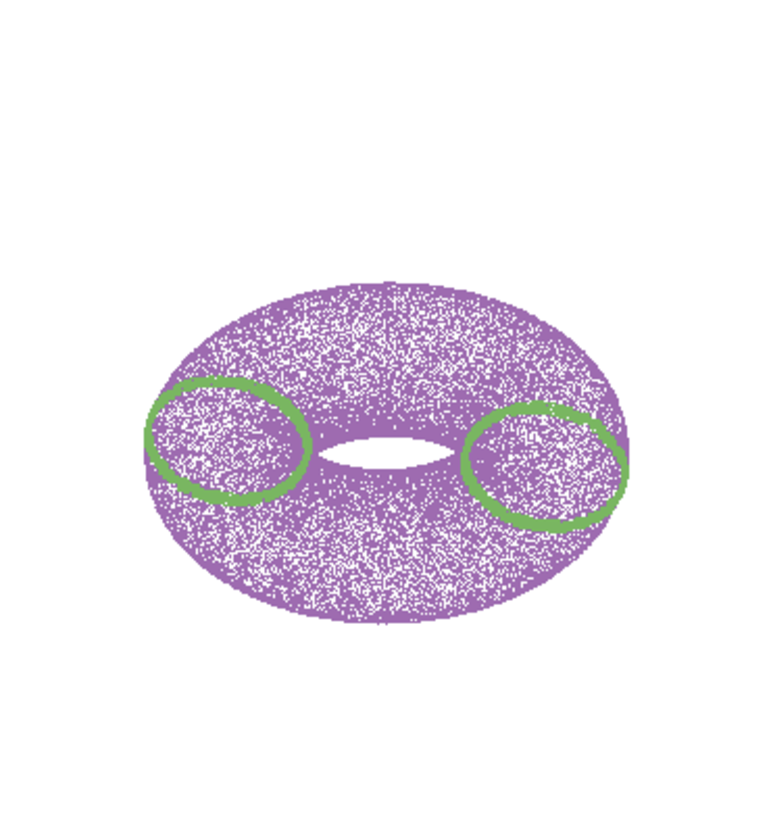
\includegraphics[width=1in]{torus-3-50k.pdf} & 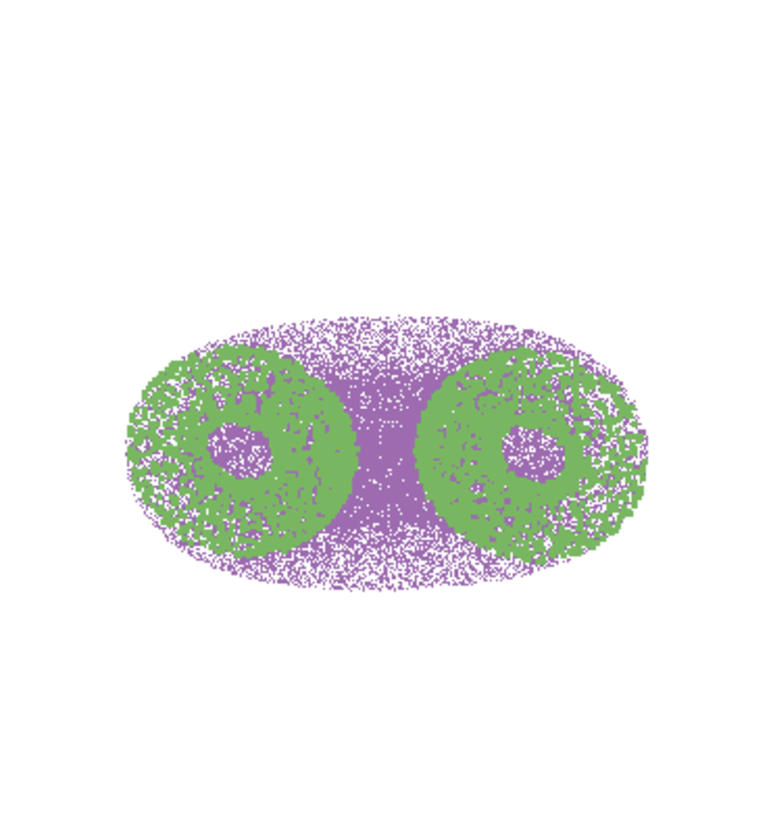
\includegraphics[width=1in]{torus-4-50k.pdf}
\end{tabular}
}
\caption{2-D, 3-D, and 4-D tori with features highlighted.}
\end{figure}

\subsection{Ring Torus} 

A ring torus has a hole in the center of the object. It is generated
recursively. A 2-D circle forms the base of the torus, which is defined by:

\begin{eqnarray*}
&&X_1: cos(t_1)r_1\\
&&X_2: sin(t_1)r_1
\end{eqnarray*}

\noindent using one radius and one angle. The 3-D torus is defined by:

\begin{eqnarray*}
&&X_1: cos(t_1)(r_1 + cos(t_2)r_2)\\
&&X_2: sin(t_1)(r_1 + cos(t_2)r_2)\\
&&X_3: sin(t_2)r_2\\
&&r_1>r_2
\end{eqnarray*}

Notice how the 3-D torus builds from the 2-D: $r_1$ is replaced by
($r_1+cos(t_2)r_2$). The 3-D torus has four parameters: two angles and
two radii. The third dimension is formed entirely by the additional
angle and radius.  A 4-D torus will be generated with the same pattern
as the 3-D torus: a new dimension will be added and material will be
inserted recursively into the formulas:

\begin{eqnarray*}
&&X_1: cos(t_1)(r_1 + cos(t_2)(r_2 + cos(t_3)r_3))\\
&&X_2: sin(t_1)(r_1 + cos(t_2)(r_2 + cos(t_3)r_3))\\
&&X_3: sin(t_2)(r_2 + cos(t_3)r_3)\\
&&X_4: sin(t_3)r_3\\
&&r_1>r_2>r_3
\end{eqnarray*}

The patterns to the higher-dimensional torus generation are:

\begin{enumerate} \itemsep 0in
\item add a new dimension each time.
\item insert material on the inside of each equation, except for the
  new dimension.
\item the newest radius will always be smaller than the previous radii.
\end{enumerate}

This is not easy to recurse, though. Inserting more material inside a
formula after it has been formed is not simple. By rearranging the
formulas, a better method is achieved:

\begin{eqnarray*}
&&X_1: ((cos(t_3)r_3 + r_2)(cos(t_2) + r_1)cos(t_1)\\
&&X_2: ((cos(t_3)r_3 + r_2)(cos(t_2) + r_1)sin(t_1)\\
&&X_3:  (cos(t_3)r_3 + r_2) sin(t_2)\\
&&X_4:   sin(t_3)r_3\\
&&r_1>r_2>r_3
\end{eqnarray*}

Here's the first step of the recursion, starting from the last
dimension.

\begin{eqnarray*}
&&X_1: cos(t_3)*r_3\\
&&X_2: cos(t_3)*r_3\\
&&X_3: cos(t_3)*r_3\\
&&X_4: sin(t_3)*r_3
\end{eqnarray*}

\noindent which translates to this R code:

\begin{verbatim}
torus<-c(
  rep(cos(t[p-1]) * radius[p-1], p-1), 
  sin(t[p-1]) * radius[p-1]
)
\end{verbatim}

From this start, we recurse backwards from $p-1$ to 2. A new radius is
added at each iteration which is multiplied with the previous equation
by the cosine of an angle. The final step adds a last radius and
multiplies the result by the sine of the new angle. 

\begin{verbatim}
for (i in (p-1):2) {
  for (j in (i-1):1) {
    torus[j]<-(torus[j] + radius[i-1])*cos(t[i-1])
  }
  torus[i]<-(torus[i]+radius[i-1])*sin(t[i-1])
}
\end{verbatim}

Here is how the recursion builds the 4-D torus:

\begin{eqnarray*}
&&p=4\\
&&Base\\
&&X_1: cos(t_3)r_3\\
&&X_2: cos(t_3)r_3\\
&&X_3: cos(t_3)r_3\\
&&X_4: sin(t_3)r_3\\
\\
&&i=p-1=3\\
&&j=2:1\\
&&X_1: (cos(t_3)r_3 + r_2)cos(t_2)\\
&&X_2: (cos(t_3)r_3 + r_2)cos(t_2)\\
&&X_3: (cos(t_3)r_3 + r_2)sin(t_2)\\
&&X_4: sin(t_3)r_3\\
\\
&&i=2\\
&&j=1:1=1\\
&&X_1: ((cos(t_3)r_3 + r_2)cos(t_2) + r1)cos(t_1)\\
&&X_2: ((cos(t_3)r_3 + r_2)cos(t_2) + r1)sin(t_1)\\
&&X_3: (cos(t_3)r_3 + r_2)sin(t_2)\\
&&X_4: sin(t_3)r_3\\
\end{eqnarray*}

This code results in one row of data for one point on the 4-D torus
for each value of angle.  By varying the angle and binding the result
we get points over the surface of the torus:

\begin{verbatim}
finished <- rbind(finished,torus.row)
\end{verbatim}

or

\begin{verbatim}
matrix(do.call("rbind", as.list(
  replicate(n, torus.row(radius,p)))),ncol=p,byrow=TRUE)
\end{verbatim}

The angles create the rings, and thus need to vary fully between 0 and
$2\pi$:

\begin{verbatim}
t <- runif(p-1,min=0,max=2*pi)
\end{verbatim}

The radii for the process are fixed at the start.  To produce a hole
in each dimension the radii need to decrease with $p$.  We set the
hole to have a size of 1 in every dimension, and the radii are a power
of 2 less than the previous dimension.

\begin{verbatim}
radius <- (2^((p - 2):0))
\end{verbatim}

\noindent This produces points fairly randomly spread on the surface of
the torus.  A more regular way to form a torus is to form the angles
into a set of intervals, resulting in more circular patterns.

\subsection{Flat Torus}

Another common hyper-torus is the flat torus. A flat torus is commonly
seen expanding into infinity as a screen saver on some computers. It
has multiple holes in the center. It is easy to generate.

A flat torus is formed in pairs of dimensions, defined by a sine and
cosine of one angle, for example the circle is generated in 2-D by
$cos(t_1)$ and $sin(t_1)$.  A flat torus in any dimension is created
from multiple pairs of sine and cosine, e.g. a 1-D torus is generated by
one pair, a 2-D torus by two pairs, four variables, and a 3-D torus by
three pairs, six variables (Figure \ref{flat1}).  All values of sine
and cosine are generated from angles, $(-2\pi, 2\pi)$, separately for
each pair.  The flat torus has an even number of dimensions, but an
effective dimension half that size. Figure \ref{flat2} illustrates the
construction.

\begin{figure}[ht]
\centerline{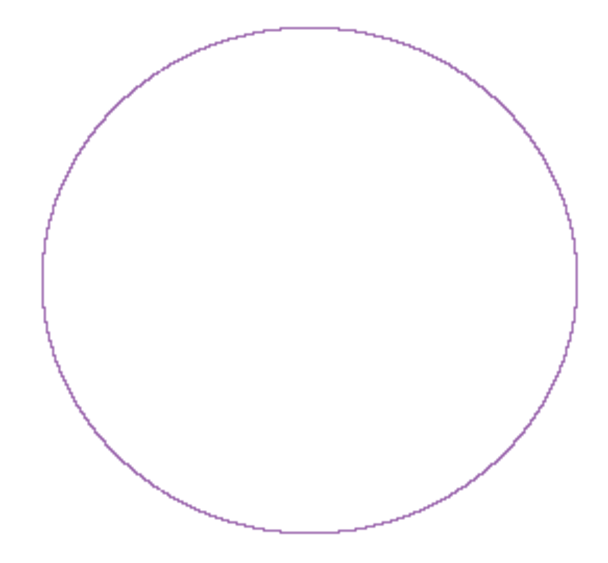
\includegraphics[width=1.3in]{torus-flat-2.pdf} \includegraphics[width=1.3in]{torus-flat-4.pdf}\includegraphics[width=1.3in]{torus-flat-6.pdf}}
\caption{Flat tori in 2-D, 4-D, and 6-D.}
\label{flat1}
\end{figure}

\begin{figure}[ht]
\centerline{\includegraphics[width=1.2in]{torus-flat-6-0.pdf} \includegraphics[width=1.2in]{torus-flat-6-1.pdf}\includegraphics[width=1.2in]{torus-flat-6-2.pdf} \includegraphics[width=1.2in]{torus-flat-6-3.pdf}}
\centerline{\includegraphics[width=4in]{torus-flat-6-matrix.pdf}}
\caption{Views of the 6-D flat tori which illustrate its
  construction. Plots 2-4 in the top row contain highlights correspond
  to those seen in the scatterplot matrix.}
\label{flat2}
\end{figure}

%\begin{figure}[ht]
%\centerline{\includegraphics[width=4in]{torus-flat-6-matrix.pdf}}
%\caption{6-D Flat Tori Matrix of Dimensions.}
%\label{flat3}
%\end{figure}

%%% Barret, can you put a reference in for this figure somewhere and
%%% explain why it is here? I think you have something to say about
%%% this but there's nothing right now.

%%%  I believe you have already referenced this picture.  ``Figure \ref{flat2} illustrates the construction.''  
%%%  It is also in the figure, that is not commented out, right above this statement.  
%%%  So, I don't think I need to reference it.

\subsection{Solid?}  %%%  Di, Why the question mark?  See if you also agree with the statement below.  Is the the smallest radii only or all but the largest?  For a doughnut it is only the smallest or all but the largest one.

These tori are all hollow. To create points in the interior of the
tori one would randomly generate the smallest radii in the hyper-ring torus and all radii in the flat torus.

\section{Conclusion}

This paper has described how \pkg{geozoo} generates several types of
high-dimensional geometric shapes. The result is a library designed to
help conceptualize high-dimensional spaces. It has also led to some
new geometric shape definitions. 

This library, although seemingly removed from real high-dimensional
data has some strong connections. Much of our data analytic methods
are based in high-dimensional Euclidean space. Developing some visual
insight into this space can help to understand the methods that
operate in the space. Some data can be closely mapped to the geometric
shapes. For example, ranked data showing preferences for a fixed set
of objects, can be mapped to high-dimensional polytopes \citep{Th93}.
Values in a sample are commonly constrained to sum to a fixed number,
for example, 100\%, forming compositional data. This type of data lies
inside a $(p-1)$-D simplex. Good experimental designs commonly have a
geometric structure \citep{HSS99}.

We encourage the reader to look at the movies, and images, and
download the data on the project web site, which is accessible from
the GGobi web site (\url{http://www.ggobi.org}). The \pkg{geozoo}
package contains the R code to generate the geometric shapes, is
available to download from CRAN (\url{http://www.R-project.org}). We
especially encourage readers to experiment with creating new
high-dimensional geometric shapes, or contribute ideas and code back to this project.

\section*{Acknowledgments}

This work was supported by National Science Foundation grant
DMS0706949. Andreas Buja provided some helpful feedback on the
work. Dianne Cook thanks the Isaac Newton Institute, Cambridge, UK for
support, where she was visiting during the last revision of this paper.

\section*{Notes}~\label{notes}

In GGobi, by default each dimension is scaled to its own local minimum
and maximum. Some objects need to be scaled to a global maximum and
minimum, e.g. an ellipsoid, to be viewed properly. To do this in GGobi
go to the Variable Manipulation Tool, and set the User Limits to be
equal to the global minimum and maximum.

\bibliography{JSS-GeometricShapes}

\end{document}
